\documentclass{llncs}

\usepackage{amsmath}
\usepackage{algorithmicx}
\usepackage{algpseudocode}
\usepackage{cite}
\usepackage{flushend}
\usepackage{graphicx}
\usepackage{graphics}
\usepackage{url}
\usepackage[table]{xcolor}
\usepackage{xspace}
\usepackage[T2A]{fontenc}

\usepackage{algorithm}
\usepackage[english]{babel}

\usepackage[utf8]{inputenc}

\newboolean{doubleblind}
\setboolean{doubleblind}{false}

\allowdisplaybreaks

\begin{document}
 We are solving the problem of the bounds on expected runtime of the evolutionary algorithm that generates test for Dijkstra algorithm such that this algorithm will relax all edges during this test.
 
 \section{First steps}
 \subsection{Experiments}
 
 First we made some experiments that calculated:
 \begin{itemize}
  \item average number of algorithm iterations depending on the number of edges with the fixed number of vertices;
  \item average number of algorithm iterations depending on the number of vertices with the fixed number of edges;
  \item average number of leaves in the generated graph during the algorihm runtime;
  \item average number of vertices in the connected component;
 \end{itemize}
 
 \subsection{Algorithm iterations}
  We made 200 algorithm runs for each number of edges and vertices and counted the number of iterations. For fixed numbers we made experiments with 5, 10 and 15 vertices and 10, 20 and 30 edges. Here are results:
  
  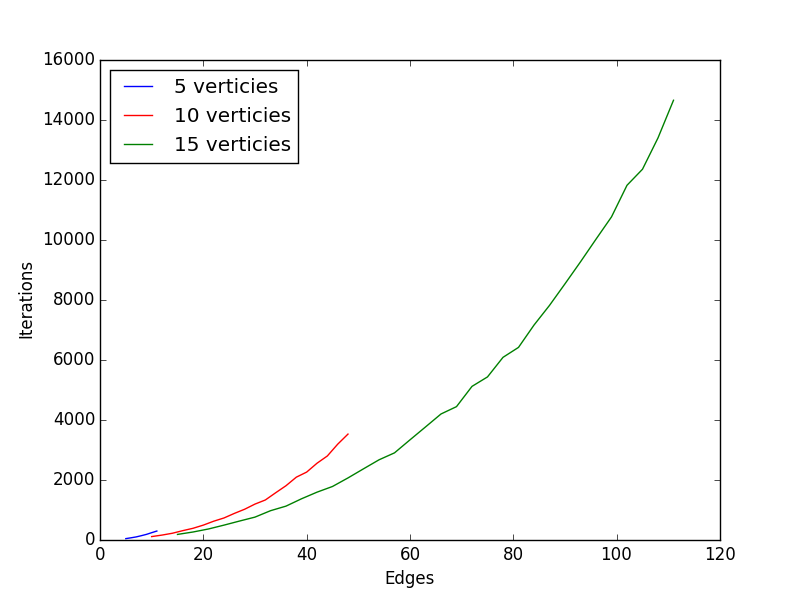
\includegraphics[height=5cm]{pic/const_vertices.png}
  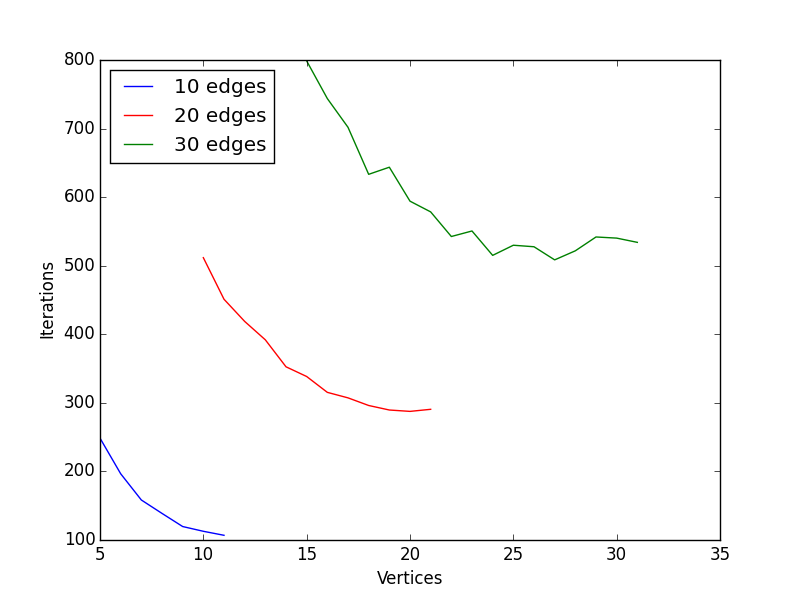
\includegraphics[height=5cm]{pic/const_edges.png}
  
  We can see that expected runtime depends straightly on the number of edges and inversely depends on the number of vertices.
  
 \subsection{First analysis}
  The algorithm run can be divided into two phases:
  \begin{itemize}
   \item the phase of growth, when all the vertices become reacheble from the start one;
   \item the phase of relaxing all edges that left unrelaxed in te first phase.
  \end{itemize}

  The analysis of the first phase is comlex because of two facts:
  \begin{itemize}
   \item in some cases size of connected component decreases by one;
   \item in some cases connected component can be extended by more than one vertex.
  \end{itemize}
  
  But we have an assumption that the first fact doesn't have much influence on the upper bound of the first phase because it's qute rare situation.
  The second fact only decreases the upper bound on runtime of the first phase.
  So we can make simple upper bound on the expectation of runtime of the first phase.
  
  The probability of the extention of the connected component by one vertex is not less then multiplication of probabilities 
  of taking the edge not from the spanning tree on the probability of putting it's new start into the connected component and it's end outside the connected component:
  
  $$P_{inc} \ge \frac{E - i + 1}{E} \cdot \frac{i(V - i)}{V^2},$$
  
  where $E$ -- number of edges, $V$ -- number of vertices in the graph, $i$ -- number of vertices in the current connected component.
  
  
  So the expectation of the extension of the connected component by one vertex is following:
  
  $$E_{inc} = P_{inc}^{-1} = \frac{EV^2}{(E - i + 1)i(V - i)}$$
  
  The expected runtime of the first phase can be calculated as the sum of expected times of extension by one vertex for every size of the connected component:
  
  \begin{align*}
   E_{i=V} & = \sum_{i = 1}^{V - 1} \frac{EV^2}{(E - i + 1)i(V - i)} = \sum_{i = 1}^{V - 1} \frac{EV}{E - i  + 1} \left( \frac{1}{V - i} + \frac{1}{i}\right) = \\
	  & = \sum_{i = 1}^{V - 1} \left( \frac{EV}{E - V + 1} \left( \frac{1}{V - i} - \frac{1}{E - i + 1} \right) + \frac{EV}{E + 1} \left( \frac{1}{i} + \frac{1}{E - i + 1} \right) \right) = \\
	  & = EV \left( \frac{1}{E - V + 1} + \frac{1}{E + 1} \right) \sum_{i = 1}^{V - 1} \frac{1}{i} + EV \left( \frac{1}{E + 1} - \frac{1}{E - V + 1} \right) \sum_{i = 1}^{V - 1} \frac{1}{E - i + 1} \approx \\
	  & \approx \frac{V(2E - V)}{E - V} \ln{V} - \frac{V^2}{E - V} (\ln{E} - \ln{(E - V)} )
  \end{align*}
  
  Here are the graphic of this functuion for $V = 500$. The red line is $2V \ln{V}$ constant that is asimptote of this function for large number of edges:
  
  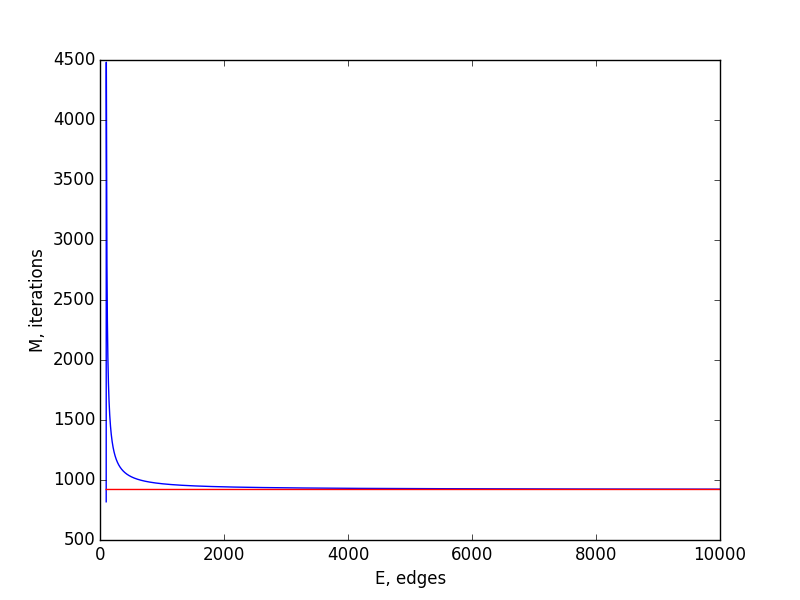
\includegraphics[height=5cm]{pic/Formula.png}
  
  We can see that with number of edges that is only little greater than number of vertices the expected runtime of the first phase is really largel. 
  But experiments showed that in this case algorithm finds optimum before the end of the first phase.
  In the next graphics we can see the average number of vertices in the connected component for each iteration. The vertical line shows the average number of algorithm iterations.
  
  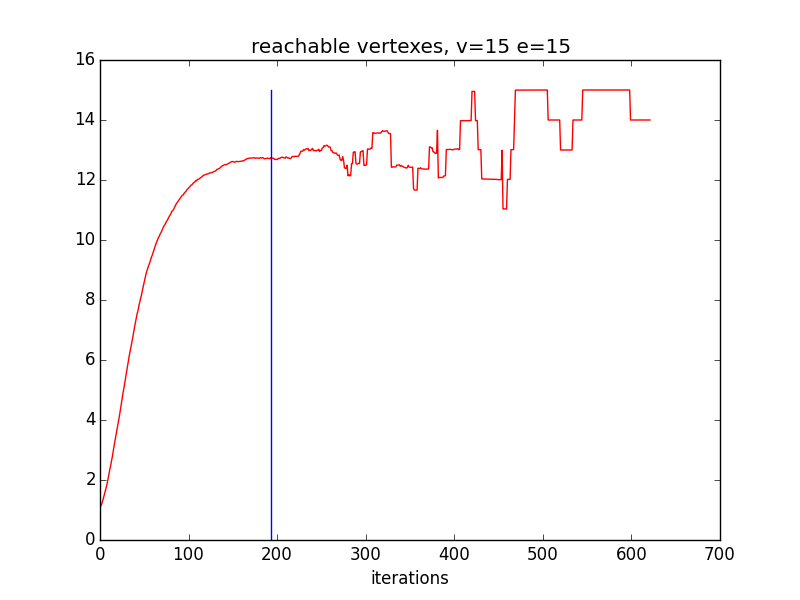
\includegraphics[height=5cm]{pic/reachable_vertices_v15e15.png}
  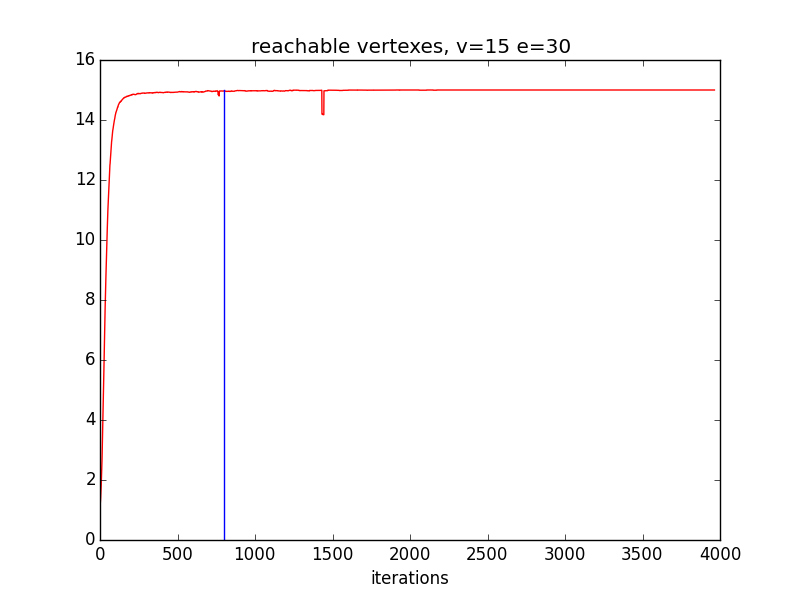
\includegraphics[height=5cm]{pic/reachable_vertices_v15e30.png}
  
  So we can see that for small number of edges the expected runtime of the algorithm is less then expected runtime of the first phase and this case should be considered separatly.
  
  Also to prove the upper bound we need to prove that the case when the size of connected component decreases is rare enough.
  But there are too many cases when the size of the component can decrease and counting their probabilities is a complex problem.
  
  %TODO посмотри дома тут формулки для листьев
  
  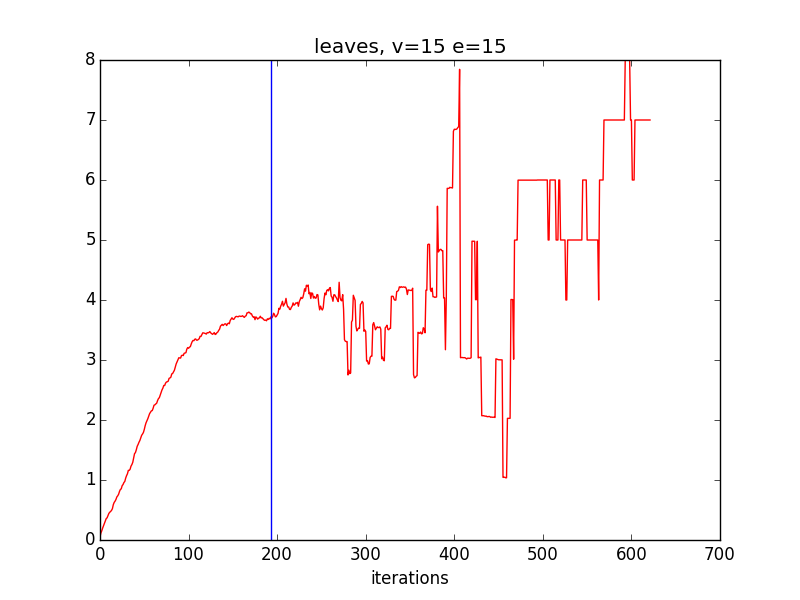
\includegraphics[height=5cm]{pic/leaves_v15e15.png}
  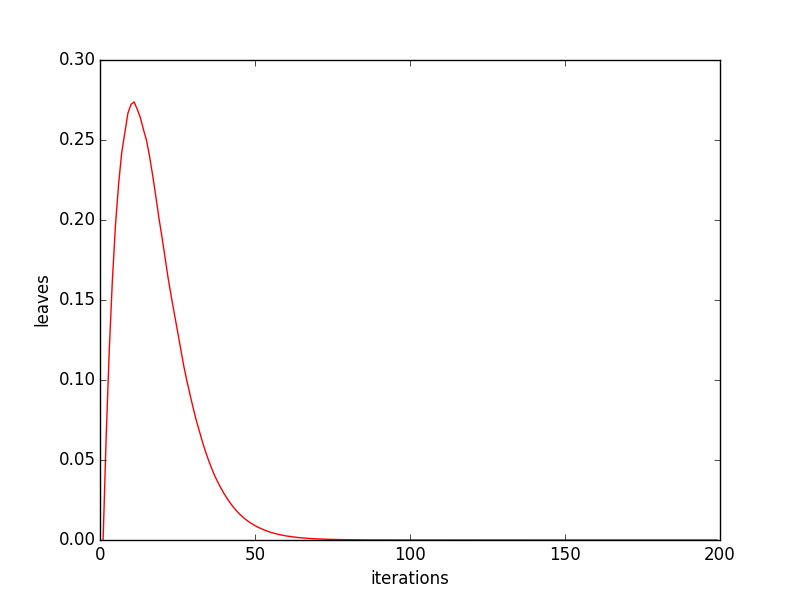
\includegraphics[height=5cm]{pic/firstPart.png}
  
 \section{Random graphs}
 \subsection{Problem statement}
  When we were talking about the simple bound on the expected runtime of the first phase, we didn't use the fact that sometimes connected component can be extended by more than one vertex. To know the expected size of extension we should answer the question: how many vertices are reachable from the start one in the randomly generated graph?
  
  Consider a graph generation procedure.
  Given $V \ge 1$, the number of vertices, and $E \ge 0$, the number of directed edges.
  We generate a graph with $V$ vertices and $E$ edges as follows. Each edge is created independently 
  of other edges. For each edge, the source and the target vertex is chosen 
  independently and equiprobably among all vertices.
  
  Our problem is, given $V$ and $E$, to evaluate the expected number of vertices that are reachable 
  through edges from a fixed starting vertex. 
  Without loss of generality we assume that we always choose the vertex $1$ as the starting vertex.
  
  The first step would be to evaluate the expected number of vertices 
  at distances $0$, $1$, \ldots, $(V - 1)$ 
  from the starting vertex and then to sum them up. To compute these expected numbers precisely,
  we use the dynamic programming technique.
  
  \subsection{First Straightforward Approach}
  
  The following dynamic programming approach will be used in this subsection:
  $A(i,v,e,l)$ is the total number of ways to place $e$ edges using $v$ vertices (including the 
  starting one) such that the maximum distance from the starting vertex is $i$ and the number of
  vertices with that distance is $l$. Here, we assume that edges are numbered, that is, we 
  distinguish the ways $[1 \to 2, 1 \to 3]$ and $[1 \to 3, 1 \to 2]$.
  
  Consider vertex sets $V_j$ consisting of vertices at the distance $j$ from the starting vertex.
  The following types of edges are allowed:
  \begin{itemize}
      \item forward edges: $u \to v$ if $u \in V_j$ and $v \in V_{j+1}$;
      \item backward edges: $u \to v$ if $u \in V_j, v \in V_k, j > k$;
      \item same-level edges: $u \to v$ if $u \in V_j$ and $v \in V_j$.
  \end{itemize}
  
  Note that forward edges may go only between ``adjacent'' vertex sets while backward edges may 
  connect non-adjacent sets as well. For the sake of simplicity, we consider backward edges and 
  same-level edges together.
  
  The initialization of dynamic programming is done for $i = 0$, i.e. when the only vertex is the 
  starting vertex. We may use arbitrary number of edges which form loops from/to the starting 
  vertex, and for every number of such edges there is only one way to do so. This results in 
  $A(0,1,e,1) = 1$ for all $0 \le e \le E$.
  
  For $A(i,v,e,l)$ when $i > 0$, consider all possible numbers $m$ of vertices at the distance of $i - 1$.
  There will be several edges from vertices from $V_{i-1}$ to vertices from $V_{i}$, in such a way that for every $v 
  \in V_{i}$ there is \emph{at least one} incoming edge. We denote the number of such edges as $e_f$.
  Additionally, there may be backward or loop edges that go from vertices from $V_i$ to $V_j$ where $j \le i$.
  We denote the number of such edges as $e_b$.
  
  We iterate over all possible values of $m$, $e_f$ and $e_b$. The number of ways to put edges at a lower level
  is $A(i-1, v-l, e-e_f-e_b)$. The number of backward and same-level edges can be simply expressed as $(lv)^{e_b}$,
  as each such edge connects a vertex from $V_i$ (there are $l$ such vertices) to any other vertex at a distance of at 
  most $i$ (there are $v$ such vertices).
  Assume that we know $B(l,m,e)$~-- the number of ways to connect $m$ vertices that constitute $V_{i-1}$ to $l$ 
  vertices that constitute $V_i$ using $e$ edges, such that every vertex from $V_i$ has at least one incoming edge.
  Apart from multiplying all mentioned quantities, we also need to consider all possible orderings of edges of 
  different types. There are $\binom{e}{e_f + e_b}$ ways to distribute additional edges among all edges, and
  $\binom{e_f + e_b}{e_f}$ ways to shuffle additional edges of two types. Finally, we need to multiply this
  by the number of ways to choose $l$ vertices.
  In total, this gives:
  
  \begin{align*}
  A(i,v,e,l)  = & \sum_{m = 1}^{v - l} \sum_{e_f = l}^{e} \sum_{e_b = 0}^{e - e_f} A(i - 1, v - l, e - e_f - e_b, m) B(l, m, e_f) (l v)^{e_b} \cdot \\ 
  & \cdot \binom{e}{e_f + e_b} \binom{e_f + e_b}{e_f} \binom{V - v + l}{l}.
  \end{align*} 
  
  \subsection{Evaluating the formulas}
  
  How to evaluate $B(l,m,e)$? We can divide all the $e$ edges in $l$ nonempty groups in $S(e, l)$ ways where $S(e, l)$ is the Stirling's number of the second kind. Edges in one group come to the same vertex from $V_i$ and we can associate each group of edges with one of the verticies in $l!$ ways. Finally for each edge we can choose starting vertex in $m$ ways. For $e$ edges there will be $m^e$ ways.
  
  As a result we have:
  $$B(l, m, e) = S(e, l) m^e l!.$$
  
  Using the exact formula for Stirling's numbers of second kind:
  
  $$B(l, m, e) = m^e \sum_{k = 0}^{l} (-1)^{l-k} k^e {l \choose k}.$$
  
  Putting it into the statement for $A(i, v, e, l)$ gives us the result:
  
  \begin{align*}
    A(i,v,e,l)  = & \sum_{m = 1}^{v - l} \sum_{e_f = l}^{e} \sum_{e_b = 0}^{e - e_f} \sum_{k = 0}^{l} (-1)^{l-k} A(i - 1, v - l, e - e_f - e_b, m) \cdot \\ 
    & \cdot (l v)^{e_b} (km)^{e_f} \binom{e}{e_f + e_b} \binom{e_f + e_b}{e_f} \binom{V - v + l}{l} \binom{l}{k}.
  \end{align*} 
  
  Now let $e_o$ be $e_b + e_f$ -- the number of edges that are used in the outward layer $V_i$. It will has values from $l$ to $e$. Then $e_b$ will be from $0$ to $e_o - l$:
  
  \begin{align*}
  A(i, v, e, l) = & \sum_{m = 1}^{v - l}\sum_{e_o = l}^{e}\sum_{e_b = 0}^{e_o - l}\sum_{k = 0}^{l} (-1)^{l - k} A(i - 1, v - l, e - e_o, m) \\
  &  {e \choose e_o} {e_o \choose e_b} {V - v + l \choose l} {l \choose k} (mk)^{e_o - e_b} (lv)^{e_b} = \\
  = & \sum_{m = 1}^{v - l}\sum_{e_o = l}^{e}  A(i - 1, v - l, e - e_o, m) {V - v + l \choose l} {e \choose e_o} \\
  & \sum_{k = 0}^{l} (-1)^{l - k} {l \choose k} \sum_{e_b = 0}^{e_o - l} {e_o \choose e_b} (mk)^{e_o - e_b} (lv)^{e_b}
  \end{align*}
  
  The next step will be convolution of the last line:
  $$ \sum_{k = 0}^{l} (-1)^{l - k} {l \choose k} \sum_{e_b = 0}^{e_o - l} {e_o \choose e_b} (mk)^{e_o - e_b} (lv)^{e_b}$$
  
  Maybe it can be done using the equality for Stirling numbers:
  
  $$S(n + 1, k + 1) = \sum_{j = k}^{n} {n \choose j} S(j, k)$$
  
  Because if we'll swap summation order we will get something like right part of this equation, but with some constant in the power of $e_f$:
  
  \begin{align*}
  & \sum_{k = 0}^{l} (-1)^{l - k} {l \choose k} \sum_{e_b = 0}^{e_o - l} {e_o \choose e_b} (mk)^{e_o - e_b} (lv)^{e_b} = \\
  & = m^{e_o} \sum_{e_b = 0}^{e_o - l} {e_0 \choose e_b} \left(\frac{lv}{m}\right)^{e_b} \sum_{k = 0}^{l} (-1)^{l - k} {l \choose k} k^{e_o - e_b} = \\
  & = (lv)^{e_0} \sum_{e_f = l}^{e_o} {e_o \choose e_f} \left(\frac{m}{lv}\right)^{e_f}\sum_{k = 0}^{l} (-1)^{l - k} {l \choose k} k^{e_f} = \\
  & = (lv)^{e_0} \sum_{e_f = l}^{e_o} {e_o \choose e_f} \left(\frac{m}{lv}\right)^{e_f} l! S(e_f, l) 
  \end{align*} 
  
  To find the way to convolute in the way like it's done for the Stirling numbers, we should find the proof for the equality above. It's simple if we try to proove it using combinatorics, but it's hard when we come to the operations with sums. All the steps I've manged to pass are the following:
  
  \begin{align*}
  (k + 1)! & S(n + 1, k + 1) =  \sum_{j = 0}^{k + 1} (-1) ^{k + 1 - j} \binom{k + 1}{j} j^{n + 1} = \\
  = &  \sum_{j = 1}^{k} (-1) ^{k + 1 - j} \left(\binom{k}{j} + \binom{k}{j - 1}\right) j^{n + 1}  + (k + 1)^{n + 1} = \\
  = & \sum_{j = 0}^{k - 1}(-1)^{k - j} \binom{k}{j} (j + 1)^{n + 1} - \sum_{j = 1}^{k}(-1)^{k - j} \binom{k}{j} j^{n + 1} + (k + 1)^{n + 1} = \\
  = &  (-1)^k + \sum_{j = 1}^{k - 1}(-1)^{k - j} \binom{k}{j} ((j + 1)^{n + 1} - j^{n + 1}) + (k + 1)^{n + 1} - k^{n + 1} = \\
  = & \sum_{j = 0}^{k}(-1)^{k - j} \binom{k}{j} ((j + 1)^{n + 1} - j^{n + 1})
  \end{align*}
  
  Now we just should prove that:
  
  \begin{align*}
  \frac{1}{(k + 1)!} \sum_{j = 0}^{k}(-1)^{k - j} \binom{k}{j} ((j + 1)^{n + 1} - j^{n + 1}) = \sum_{i = k}^{n} \binom{n}{i} \frac{1}{k!} \sum_{j = 0}^{k} (-1)^{k-j} \binom{k}{j} j^i.
  \end{align*}
  
  If we change the summing order of the right part, we'll recive two sums with the same number of summands, but this summands are different:
  
  \begin{align*}
  \frac{1}{(k + 1)!} \sum_{j = 0}^{k}(-1)^{k - j} \binom{k}{j} ((j + 1)^{n + 1} - j^{n + 1}) =  \frac{1}{k!} \sum_{j = 0}^{k} (-1)^{k-j} \binom{k}{j}  \sum_{i = k}^{n} \binom{n}{i} j^i.
  \end{align*}
    
  
  \subsection{Final phase}
  
  The final phase would be to find the expected number of vertices at a distance of $i$ for each $0 \le i < V$.
  To do that, we consider $A(i, v, e, l)$ for all $1 \le v \le V$, $0 \le e \le E$, $0 \le l \le v$
  and evaluate the number of ways to put the remaining edges which do not break the assigned distances.
  More precisely, we need to put $E - e$ edges which either:
  \begin{itemize}
  \item go from $V_i$ to unconsidered vertices;
  \item go from unconsidered vertices to $V_j$ where $0 \le j \le i$;
  \item connect unconsidered vertices.
  \end{itemize}
  
  Two latter cases can be merged to make $V (V - v)$ ways to put an edge. The former case
  produces $l (V - v)$ ways, which is $(V - v) (V + l)$ ways in total. 
  This results in $((V - v) (V + l))^{E-e}$ ways to choose remaining edges, additionally,
  we need to shuffle them with existing edges, which requires a multiple of $\binom{E}{e}$.
  So, if $C(i,l)$ is the number of ways to have $l$ vertices at a distance of $i$, then:
  
  $$C(i,l) = \sum_{v = 1}^{V} \sum_{e = 0}^{E} \sum_{l = 0}^{v} A(i,v,e,l) ((V - v)(V + l))^{E - e} \binom{E}{e}.$$
  
  The total number of graphs is $V^{2E}$, so the expected number of vertices at a distance of $i$ is:
  
  $$E(i) = \sum_{l=0}^{V} \frac{C(i,l) \cdot l}{V^{2E}}.$$
  
  The following resources are needed to compute $E$ using the proposed method:
  \begin{itemize}
  \item evaluation of $B$: $O(V)$ time, $O(1)$ memory;
  \item evaluation of $A$: $O(V^4 E^3)$ time, $O(V^3 E)$ memory;
  \item evaluation of $C$: $O(V^4 E)$ time,   $O(V^2)$ memory;
  \item evaluation of $E$: $O(V^2)$ time,     $O(V)$ memory.
  \end{itemize}
  
  The required memory for $A$ can be reduced $O(V)$ times without any effort 
  as we need only $A(i, \ldots)$ and $A(i - 1, \ldots)$ at once.
  The $C$ array can be optimized out as it is introduced for clarity only.
  However, the time for $A$, which is $O(V^4 E^3)$, clearly dominates over all stages of this approach.
 
 
\end{document}
